As our goal is to achieve high re-usability, modularity and openness, we built our software architecture on the Robot Operating System (ROS) middleware, using version Indigo \cite{ros} running on Ubuntu Trusty Tahr. 
Additionally, our system uses some of the publicly released packages from the STRANDS project \cite{strands}. 
This allows us to not only integrate the cutting edge research to our robot, but also to contribute to the evaluation of this research. 
Moreover, we integrate our own research where our interest overlaps with the focus of the competition.
Our system architecture contains the following modules.

\subsection{State machine}

Even though AI planning is in our expertise, we use \textit{finite state machines} to control and monitor the robot's states and actions. 
We have two main reasons for this decision. First, the competition defines all \textit{task benchmarks} as short scripts, so a robot does not have too much freedom in decisions on how to fulfil a task. Second, a state machine provides us with \textit{repeatability} during testing.


For each of the benchmarks, we develop the state machine using ROS's SMACH package, that is ``a task-level architecture for rapidly creating complex robot behaviour" \cite{smach}. 
All of the task's state machines are linked with the central state machine which communicates with the referee box and based on the accepted benchmarking test triggers specific state machines. 

\subsection{Navigation}

We use standard ROS packages for localisation, mapping and low-level navigation, e.g. navigation planning a path from the initial coordinates to the goal coordinates. 
We observed that in some cases, such as passing narrow doors and passing through a doorway, a special robot behaviour would be better. 
Therefore, we are extending our system using high-level topological navigation \cite{jaime} and we can strongly benefit from three main features:

\begin{itemize}
\item Waypoints and edges are managed in a database which allows even online modification.  
\item A special robot behaviour can be specified on the edges overriding standard move-base.
\item A navigation policy \cite{bruno} provides paths on the top of the topological map containing waypoints. 
\end{itemize}
Thus, the robot must pass the surrounding area of the waypoint on the path. This can be mainly used to demand certain robot movements and keep the robot away from obstacles in an environment.



\subsection{Mapping} is done by \textit{OpenSlam's GMapping} algorithm \cite{slam} through the ROS wrapper package called \textsf{slam gmapping}. This approach uses a Rao-Blackwellized particle filter in which each particle carries an individual map of the environment. The particles are updated by taking into account both odometry and the latest observations from a laser range finder.

\subsection{Localisation} in a known map uses an \textit{Adaptive Monte Carlo Localization} (AMCL)\cite{amcl} algorithm. This node is part of the ROS \textsf{navigation stack} package. It uses laser range finder readings to update a particle filter. Every particle represents a specific discrete state and stores the uncertainty of the robot being in that state/position within the known map. Also, every time the robot moves it uses the motor information to shift the particles to the corresponding direction.

\subsection{Low-level navigation using move-base} was used last year as the only navigation system. It is a proven robust solution for domestic environments \cite{Marder-Eppstein2010}. More specifically this node reads the odometry, the current pose estimate and the laser range finder scans and 3-D points clouds from a depth camera and safely drives the robot in the environment to a predefined goal. In order to navigate smoothly, it uses a combination of a global and a local planner. The global planner creates an optimal global path based on the robot's pose and a global cost-map. Then the local planner, which uses the \textit{Dynamic Window Approach} algorithm \cite{dwa}, is responsible for following the global path and reactively avoiding obstacles. 

\subsection{\label{sec:vision}Face detection and recognition}

Face detection, see Fig. \ref{fig:face}, is performed using the \textit{Viola-Jones} algorithm \cite{Viola01_RapidObjDet}. The algorithm looks for faces by incrementally applying many simple Haar classifiers. The composition is performed by a cascade function, which needs to be trained \textit{a priori} with many positive and negative images. The resulting classifier can find faces efficiently and independent of the size of the faces and light conditions.

Face recognition is performed by applying a \textit{Local Binary Pattern Histogram} (LBPH) algorithm \cite{Ahonen04_FaceRecLBP}. The principle of the algorithm is to build local binary patterns (LBP) for each pixel depending on a variable neighbourhood scheme. Then, it divides the formed LBP image into $m$ local regions and computes the LBP distribution histogram from each region. Finally, classification is performed by comparison between the LBP histograms of a new face with the ones from the dataset.

\begin{figure}[!t]
\centering
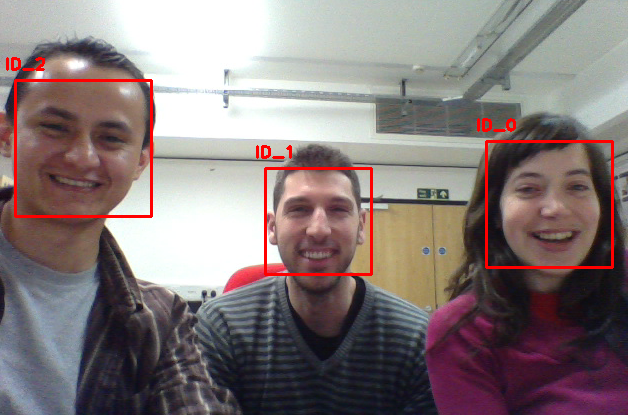
\includegraphics[width=3.in]{BARC_FaceRec.png}
\caption{An example of the face detection and face recognition algorithms. The red bounding boxes surround the successfully detected faces, while each of them is given a corresponding identification code.}
\label{fig:face}
\end{figure}

\subsection{Uniform Detection}

Our uniform recognition uses colour segmentation of an input image in to two regions. 
A positive region corresponds to a colour within previously manually calibrated lower and upper bounds. 
In contrast, a negative region corresponds to the colours outside of these limits. 
Based on the size of the positive region, the person is classified as a Postman, Deliman or other. 









